\chapter{Аналитический раздел}
В аналитическом разделе формализованы задачи и объекты сцены, определены геометрические и оптические характеристики объектов сцены. Также проанализированы и описаны алгоритмы, используемые для визуализации и генерации ландшафтной сцены с облаками. Установлены допустимые диапазоны и ограничения, накладываемые на входные данные.

\section{Формализация задачи и объектов}

Объектами сцены являются:
\begin{enumerate}
	\item облака;
	\begin{itemize}
		\item высота, на которой находятся облака;
		\item ширина: горизонтальное пространство, которое облака занимают на небе;
		\item скорость движения облаков в горизонтальной плоскости;
		\item кучность: степень сгущённости и концентрации облаков, что влияет на их внешний вид и отбрасываемую тень.
		\item плотность: определяет, сколько солнечного света облака могут заблокировать, что влияет на освещённость ландшафта.
	\end{itemize}
	\item ландшафт;
	\begin{itemize}
		\item рельеф: равнина --- земная поверхность без гор и значительных холмов~\cite{ushakov};
		\item материалы и текстуры: характеристики поверхности, такие как цвет и диффузное отражение.
	\end{itemize}
	\item бесконечно удаленный источник света (солнце);
	\begin{itemize}
		\item расположение: определяется азимутальным и зенитным углом на небесной сфере от $0^{\circ}$ до $180^{\circ}$.
		\item интенсивность: яркость, с которой будет освещена сцена.
	\end{itemize}
	\item наблюдатель (камера).
	\begin{itemize}
		\item расположение: координаты и угол обзора камеры, позволяющие наблюдать сцену с разных ракурсов;
		\item поле зрения: угол обзора, влияющий на ширину сцены.
	\end{itemize}
\end{enumerate}

\section{Оптическая модель облаков}
\subsection{Закон Бугера~---~Ламберта~---~Бера}
Для облаков некоторая часть света рассеивается от направления распространения, а еще большее количество поглощается каплями воды и молекулами озона, но остается часть, которая продолжает движение без изменений~\cite{guerrilla_volumetric_cloudscapes_2023, sym10040125}.

\textit{Закон Бугера---Ламберта---Бера} определяет ослабление пучка света при поглощении средой.
\begin{equation}
	\label{eq:beers-law}
	I_l=I_{o}e^{-k_{\lambda }l},
\end{equation} где 
{$I_{0}$} -- интенсивность света на входе в вещество, 
$l$ -- расстояние, прошедшее светом,
$k_\lambda$ -- показатель поглощения среды.

\subsection{Фазовая функция Хеньи -- Гринстейна}
Облака представляют собой анизотропную среду (среда, где физические свойства: показатели преломления, скорость распространения и пр. -- различаются в различных направлениях внутри этой среды) из-за того, что облака представляют собой капли жидкой воды и кристаллов ледяного льда~\cite{windahl_real_time_2018}. Для описания этого используют фазовую функцию (индикатриса) Хеньи -- Гринстейна~\cite{guerrilla_volumetric_cloudscapes_2023, sym10040125}

\textit{Фазовая функция Хеньи -- Гринстейна} определяет угловое распределение интенсивности для наблюдателя:
\begin{equation}
	\label{eq:henyey-greenstein}
	P(g, \theta) = \frac{1 - g^2}{(1 + g^2 - 2g \cos\theta)^{3/2}}
\end{equation} где 
$\theta$ --  угол между направлением распространения света и взгляда наблюдателя и $g$ -- параметр асимметрии, который описывает среднее значение косинуса угла рассеяния.

\section{Алгоритмы визуализации облаков}
Существует несколько подходов к реализации облаков \cite{unigine_volumetric_clouds_2022,guerrilla_volumetric_cloudscapes_2023,  sym10040125}:	\begin{itemize}
\item геометрический: облака представляют собой, например, набор треугольников, сфер или прямоугольников. Геометрический подход к созданию облаков имеет смысл для создания изображения в определённой стилистике (Рисунок~\ref{fig:clouds}~(a))~\cite{unigine_volumetric_clouds_2022};
\item двумерная текстура: простой и малозатратный подход, но такая статичная картинка имеет смысл только как дальнеплановые статичные изображения, через которые, например, нельзя пролететь сквозь. К тому же, такие облака не могут отбрасывать тени \cite{unigine_volumetric_clouds_2022};
\item объемные \textit{(volumetric)}: динамические облака, с которыми можно взаимодействовать и которые способны отбрасывать тени (Рисунок~\ref{fig:clouds}~(б))~\cite{shadows2023, guerrilla_volumetric_cloudscapes_2023}. Именно поэтому такие облака будут реализованы в данной работе.
\end{itemize}
\begin{figure}[h!]
	\centering
	\begin{minipage}{0.48\textwidth}
		\label{fig:minecraft}
		\centering
		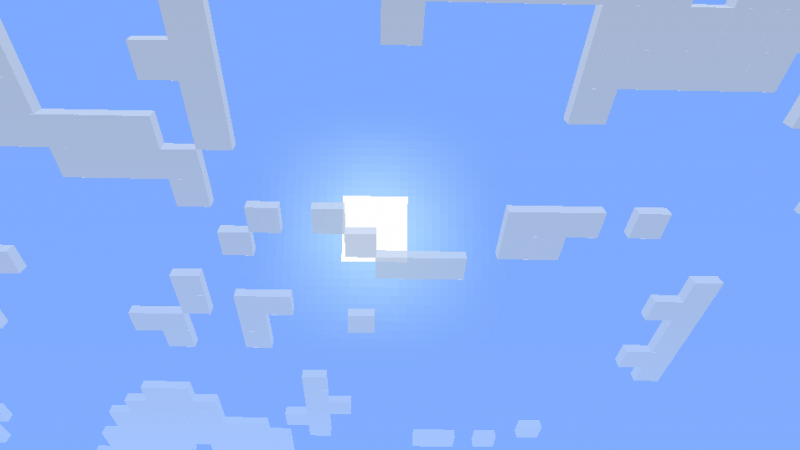
\includegraphics[width=\textwidth]{minecraft.png}
		\caption*{а}
	\end{minipage}
	\hfill
	\begin{minipage}{0.48\textwidth}
		\label{fig:unigine_volumetric_clouds_2022}
		\centering
		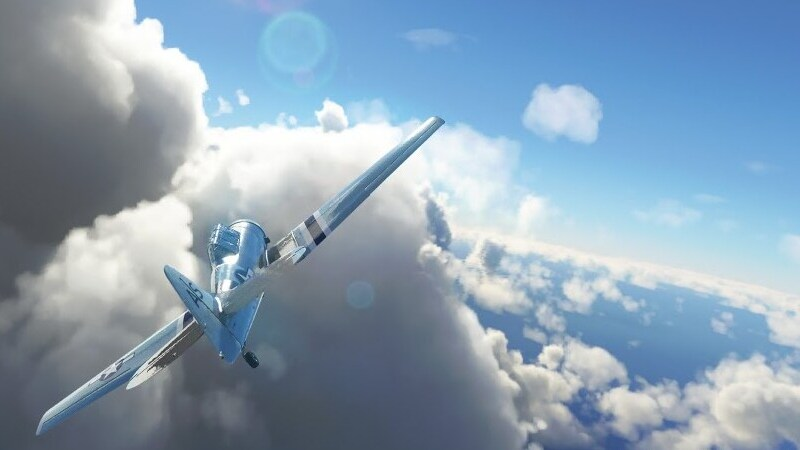
\includegraphics[width=\textwidth]{mfs.jpg}
		\caption*{б}
	\end{minipage}
	\caption{(а) геометрические облака в компьютерной игре \textit{Minecraft};\\ (б) объёмные облака в компьютерном авиасимуляторе \textit{Microsoft Flight Simulator}}
	\label{fig:clouds}
\end{figure}


Исходя из требований к алгоритму, выдвигаемых в современной игровой индустрии \cite{unigine_volumetric_clouds_2022,guerrilla_volumetric_cloudscapes_2023,  sym10040125}, условия, которые будут использованы в данной работе:
\begin{itemize}
	\item облака должны быть объемные;
	\item облака должны генерироваться процедурно;
	\item алгоритм должен быть быстродействующим.
\end{itemize}
\subsection{Жидкостная симуляция} 

Использование жидкостной симуляции для создания объемных облаков: создать простые объекты (сферы, шары), вокселизировать их и рассматривать их как жидкость, получая похожие на объемные облака фигуры \cite{guerrilla_volumetric_cloudscapes_2023}.
Современные физические модели облаков, основаны на решении \textit{уравнений Навье-Стокса}~\cite{sym10040125}, что влечет за самой следующие недостатки~\cite{sym10040125}:
\begin{itemize}
	\item алгоритм медленный;
	\item сложность контроля генерации;
	\item сложность реализации.
	
Из-за этих недостатков не используется в индустрии компьютерной графики, например в игровой~\cite{unigine_volumetric_clouds_2022}.
\end{itemize}
\subsection{Воксельная генерация}
Алгоритм заключается в генерации ограничивающего параллелепипеда (bounding box), состоящего из вокселей, хранящих информацию о цвете~\cite{guerrilla_volumetric_cloudscapes_2023}.
Преимущества:
\begin{itemize} 
	\item хорошо сочетается с алгоритмом построением теней
\end{itemize}
Недостатки: 
\begin{itemize} 
	\item высокие затраты памяти; 
	\item сложность обработки большого количества вокселей в реальном времени; 
	\item необходимость оптимизаций для обработки больших объемов. 
	
Из-за этих недостатков так же не используется в индустрии компьютерной графики, например в игровой~\cite{unigine_volumetric_clouds_2022}.
\end{itemize}
\subsection{Визуализация на основе трассировки лучей}
В алгоритме также используется ограничивающий параллелепипед, у которого визуализируются пиксели, соответствующие его видимым граням.
Вместо вычисления каждого вокселя, алгоритм из точки наблюдателя для пикселя, соответствующему видимой грани параллелепипеда высчитывает его итоговый цвет~\cite{Patapom2013, sym10040125}. 

Для получения итогового цвета используется трёхмерная текстура сгенерированного шума~\cite{guerrilla_volumetric_cloudscapes_2023}.
\newpage
\begin{figure}[htb!]
	\centering
	\includesvg[width=0.5\textwidth]{cloud.svg}   
	\caption{Генерация на основе обратной трассировки лучей}
	\label{fig:my_label}
\end{figure}

Так для каждого луча вычисляется накопленная из шума плотность (Рисунок~\ref{fig:cloud-sampling} демонстрирует трассу луча). Накопленная плотность преобразуется в интенсивность пикселя по закону Бугера~\ref{eq:beers-law}.
\begin{figure}[htb!]
	\centering
	\includesvg[width=0.6\textwidth]{cloud_sampling.svg}   
	\caption{Получение плотности облака лучом. Крестики -- точки, в которых значения текстуры облака используются для вычисления плотности.}
	\label{fig:cloud-sampling}
\end{figure}


Визуализация на основе обратной трассировки лучей показывает преимущество перед воксельной и жидкостной генерациях, так как обрабатывает пиксели, соответствующие видимым граням ограничивающего параллелепипеда, что снижает вычислительные затраты и экономит память, что необходимо при формировании динамического изображения.
Алгоритм рекомендован к использованию на практике~\cite{guerrilla_volumetric_cloudscapes_2023, sym10040125, windahl_real_time_2018}.

\section{Способы представления ландшафта}
\subsection{Аппроксимация примитивами}
Для представления сгенерированного ландшафта используются примитивы, и наиболее распространенным и простым вариантом являются треугольники~\cite{hirnschall_perlin_2024}.

Также используется высотная карта -- это двумерная текстура, где каждое значение соответствует высоте точки на поверхности. 

Формируется сетка, состоящая из вершин, соединенных ребрами. Каждая вершина соответствует точке в высотной карте, а ребра образуют треугольники.

\subsection{Аппроксимация неявными кривыми}
Неявная кривая -- это функция $F(x, y) = 0$, где равенство не выражает ни решение x от переменной y, ни наоборот.
В частности, используются кривые, использующие тригонометрические функции.
Тогда рельефом будет служить кривая, построенная по этой функции~\cite{bird2013techniques}.

Подбор коэффициентов для получения такой кривой делает этот способ менее гибким и сложно контролируемым, чем использование предыдущего метода с использованием двумерной текстуры. 

\section{Шумы для процедурной генерации}
Для моделирования объемных облаков используются трёхмерные текстуры, для создания форм, напоминающих облака~\cite{windahl_real_time_2018}. Аналогичные текстуры используются для получения рельефа.

В работе рассматриваются два шума: Перлина и Ворли~---~Вороного. Существуют и другие шумы, однако использование конкретного шума для получения облаков и рельефа не является критичным и часто зависит только от визуальных и эстетических предпочтений. В данной работе для рельефа выбран шум Перлина, а для облаков -- Ворли~---~Вороного. 
\subsection{Шум Перлина}
Шум Перлина (Рисунок~\ref{fig:noise-images} (а)) -- это пример градиентного шума~\cite{hirnschall_perlin_2024}. Он не содержит полностью случайных значений в каждой точке, а представляет собой <<волны>>. На рисунке~\ref{fig:perlin-xy-image} представлен пример такой <<волны>>, чьи значения постепенно увеличиваются и уменьшаются. Ввиду этого, такой шум часто  используется для создания рельефа.
\begin{figure}[htb!]
	\centering
		\includesvg[width=1.0\textwidth]{perlin_xy.svg}
		\caption{Шум Перлина}
		\label{fig:perlin-xy-image}
\end{figure}


Для получения функции этого шума $p(x): \mathbb{R}^n \rightarrow \mathbb{R}^n \in [0, 1]^n$ необходим набор векторов из псевдослучайных чисел $g_u \in \mathbb{R}^n$ и значений $u \in \mathbb{Z}^n$ и, учитывая, что $p'(u) = g_u$ и $p(u) = 0$, остальные значения получаются путём интерполяции.
\subsection{Шум Ворли~---~Вороного}
Шум Ворли~---~Вороного (Рисунок~\ref{fig:noise-images} (б)) позволяет получить круглые, пузыреподобные формы, напоминающие облачные структуры~\cite{guerrilla_volumetric_cloudscapes_2023, thebookofshaders_cellular_noise_2024}.

Для получения функции этого шума $w(x): \mathbb{R}^n \rightarrow \mathbb{R}^n \in [0, 1]^n$: необходим набор из $m$ векторов псевдослучайных чисел $g_i \in \mathbb{R}^n, i \in 1, 2, \ldots, m$.

Тогда $w(x) = \underset{i \in 1, 2, \ldots, m}{\min \left( \rho(x, g_i) \right)}$, где $\rho(x, y)$ -- расстояние между x и y. Далее значения $w(x)$ нормализуются по максимальному значению.

\begin{figure}[htb!]
	\centering
	\begin{minipage}{0.48\textwidth}
		\centering
		\includesvg[width=0.6\textwidth]{perlin.svg}
		\caption*{а}
	\end{minipage}
	\hfill
	\begin{minipage}{0.48\textwidth}
		\centering
		\includesvg[width=0.6\textwidth]{worley.svg}
		\caption*{б}
	\end{minipage}
	\caption{(а) шум Перлина; (б) шум Ворли}
	\label{fig:noise-images}
\end{figure}

\section{Модель освещения}
\subsection{Модель Фонга}
Интенсивность зеркального отраженного света (рисунок~\ref{fig:phong}) зависит от угла падения, длины волны падающего света и свойств вещества~\cite{rodgers1989algorithms}. Зеркальное отражение -- направленное. Угол отражения от идеально отражающей поверхности равен углу падения. Это значит, что угол наблюдения совпадает с углом отражения. При неидеальных поверхностях, количество света достигшего наблюдения зависит от пространственного распределения отраженного света. У гладких поверхностей распределенное узкое, у шероховатых -- более широкое. Благодаря зеркальному отражению появляются световые блики~\cite{rodgers1989algorithms}.
\begin{figure}[ht!]
	\centering
	\includesvg[width=0.5\textwidth]{phong.svg}   
	\caption{Зеркальное отражение: $\vec{V}$ — вектор наблюдения, $\vec{P}$ — отраженный луч, $\vec{L}$ — падающий луч и $\vec{N}$ нормаль к поверхности.} 
	\label{fig:phong}
\end{figure}

В моделе Фонга используют эмпирическую форму~\cite{rodgers1989algorithms}:
\begin{equation}
	\label{eq:phong}
	I = I_lw(i,\lambda)\cos^n(\theta),
\end{equation}
где $I$ -- интенсивность отраженного света, $I_l$ -- интенсивность точечного источника, w(i, $\lambda$) -- кривая отражения, представляющее отношение зеркального отраженного света, к падающему как функцию угла падения $i$ и длины волны $\lambda$, n -- степень, аппроксимирующая пространственное распределение зеркального света.
\subsection{Модель Ламберта}
Диффузное отражения происходит, когда свет проникает под поверхность объекта, поглощается, а затем вновь испускается (Рисунок~\ref{fig:lambert})~\cite{rodgers1989algorithms}. 
\begin{figure}[ht!]
	\centering
	\includesvg[width=0.5\textwidth]{lambert.svg}   
	\caption{Диффузное отражение: $\vec{L}$ — падающий луч и $\vec{N}$ нормаль к поверхности.}
	\label{fig:lambert}
\end{figure}

Не зависит от положения наблюдателя, так как рассеивается равномерно по всем направлениям~\cite{rodgers1989algorithms}.
Интенсивность отраженного света вычисляется по закону косинусов Ламберта:
\begin{equation}
	\label{eq:lambert}
	I = I_lk_d\cos(\theta),
\end{equation}
где $I$ -- интенсивность отраженного света, $I_l$ -- интенсивность точечного источника, $k_d$ -- коэффициент диффузного отражения, $\theta$ -- угол между направлением света и нормалью к поверхности.

Поверхность с ламбертовым диффузным отражением выглядит матовой и блеклой~\cite{rodgers1989algorithms}, что имеет смысл для изображения травяного рельефа.
Так как рельеф~--~незеркальная поверхность, в работе используется модель Ламберта.

\section{Учёт теней от облаков на поверхности}
Тени от облаков зависят только от положения источника света и не зависят от положения наблюдателя~\cite{rodgers1989algorithms}. Для объемных облаков при построении их теней аналогично используется обратная трассировка лучей: при движении луча от поверхности к облакам определяется суммарная
плотность облаков по пути, чтобы вычислить, сколько света блокируется~\cite{shadows2023}.

Таким образом, учитывая закон Бугера--Ламберта--Бера~\ref{eq:beers-law} и закон Ламберта~\ref{eq:lambert}, итоговая формула для расчета интенсивности света на поверхности:
\begin{equation}
	I_s = I_0 I_l k_d \cos(\theta) e^{-k_{\lambda} l}.
\end{equation}

\section{Удаление невидимых линий и поверхностей}
\subsection{Алгоритм Робертcа}

Алгоритм Робертса — метод работающий в объектном пространстве. Алгоритм прежде всего удаляет из каждого тела те ребра или грани, которые экранируются самим телом. Затем каждое из видимых ребер каждого тела сравнивается с каждым из оставшихся тел для определения того, какая его часть или части, если таковые есть, экранируются этими телами~\cite{rodgers1989algorithms}. 

\subsection{Алгоритм Варнока}

Алгоритм работает в пространстве изображения~\cite{rodgers1989algorithms}. Алгоритм разбивает окно, чтобы определить, является ли его содержимое достаточно простым для отрисовки, если нет -- рекурсивно разбивает его дальше~\cite{rodgers1989algorithms}.


\subsection{Алгоритм Вейлера-Азертона}

Оптимизация алгоритма Варнока в отношении числа выполняемых разбиений за счёт перехода от прямоугольных разбиений к разбиениям вдоль границ многоугольников. Работает в пространстве изображений~\cite{rodgers1989algorithms}.

\subsection{Алгоритм художника}

Используется для простых элементов сцены, например для многоугольников~\cite{rodgers1989algorithms}. Алгоритм аналогичен тому способу, которым художник создает картину. Сначала художник рисует фон, затем предметы, лежащие на среднем расстоянии, и, наконец, передний план. Тем самым художник решает задачу об удалении невидимых поверхностей, или задачу видимости, путем построения картины в порядке обратного приоритета~\cite{rodgers1989algorithms}.

\subsection{Метод обратной трассировки лучей}
В этом алгоритме предполагается, что сцена уже преобразована в пространство изображения~\cite{rodgers1989algorithms}. 

Алгоритм работает за счет отслеживания (трассировки) лучей от наблюдателя к объекту. Трассировка прекращается, как только луч пересекает поверхность видимого объекта. 

\subsection{Алгоритм, использующий Z-буфер}
Z-буфер -- хранит значения глубины \( z \) для каждого пикселя~\cite{rodgers1989algorithms}.

\subsubsection*{Этапы работы алгоритма}

\begin{enumerate}
	\item Инициализация Z-буфера минимально возможным значением \( z \).
	\item Преобразование каждого многоугольника сцены в растровую форму.
	\item Для каждого пикселя \((x, y)\), принадлежащего многоугольнику, вычисляется его глубина \( Z(x, y) \).
	\item Выполняется сравнение глубины \( Z(x, y) \) с текущим значением глубины \( Z_{\text{буф}}(x, y) \), хранящимся в Z-буфере. Если $Z(x, y) > Z_{\text{буф}}(x, y)$,
	то в буфер кадра записывается атрибут пикселя (цвет) и значение \( Z_{\text{буф}}(x, y) \) заменяется на \( Z(x, y) \).
\end{enumerate}

Так как для визуализации облаков используется алгоритм обратной трассировки лучей, работающий непосредственно с пикселями, а не в объектном пространстве, следует выбрать алгоритм, работающий в пространстве изображений.

Ввиду простоты реализации из рассмотренных был выбран алгоритм, использующий~Z-буфер.

\section{Методы закраски}
\subsection{Простая закраска}

Вся грань закрашивается единственным цветом, интенсивность которого рассчитывается по закону Ламберта~\ref{eq:lambert}. Простая закраска используется при выполнении трех условий~\cite{kurov2024lections}:
\begin{itemize}
	\item источник находится в бесконечности: так как падающие лучи параллельны друг другу -- это повлияет на расчёт диффузной составляющей, так как она зависит от угла падения, однако для всех точек угол падения одинаков, значит диффузная составляющая одинакова;
	\item закрашиваемая грань является реально существующей, а не полученной в результате аппроксимации поверхности;
\end{itemize}

Так как рельеф, который закрашивается в работе будет получен с помощью аппроксимации, простая модель не будет использоваться в этой работе.

\subsection{Закраска методом Гуро}
При такой закраске определяется интенсивность в вершинах на основе нормали к вершине как среднее нормалей граней, образующих эту вершину, а затем интерполяцией вычисляется интенсивность каждого пикселя многоугольника~\cite{rodgers1989algorithms}.

\subsection{Закраска методом Фонга}
При такой закраске определяются нормали в вершинах многоугольника, а затем интерполяцией вычисляется нормаль каждого пикселя многоугольника, а затем его интенсивность.
При таком методе достигается лучшая аппроксимация поверхности~\cite{rodgers1989algorithms}. Именно по этому критерию этот метод выбран для закраски ландшафта.

\section*{Вывод}
В аналитической части формализованы задачи и объекты сцены. Также проанализированы и описаны алгоритмы, используемые для визуализации ландшафтной сцены с облаками. 	
Был выбран алгоритм использующий обратную трассировку лучей для визуализации объемных облаков, а также метод представления ландшафта с помощью аппроксимацией примитивами. Для процедурной генерации ландшафта выбран шум Перлина, для облаков -- Ворли~---~Вороного.

Описана оптическая модель облаков и выбраны алгоритмы решения основных задач компьютерной графики. Для удаления невидимых линий и поверхностей выбран алгоритм использующий Z-буфер. Для учёта теней и освещения рассмотрены и выбраны закон ламбертового диффузного отражения и закраска методом Фонга.
